\section{Task3 --- Encryption Mode --- ECB vs. CBC}
%

\begin{figure}
    \centering
    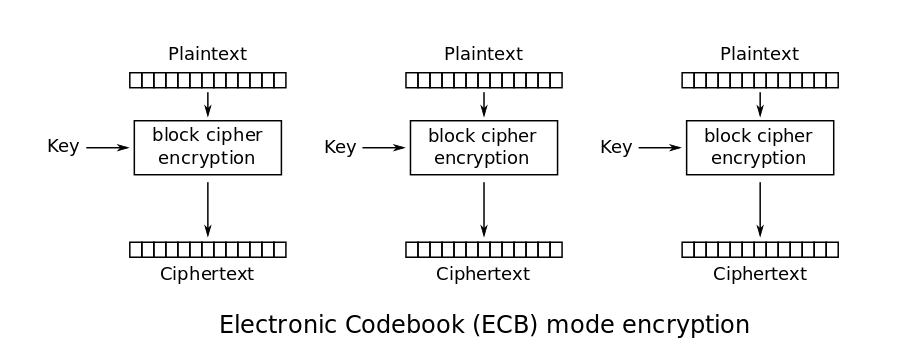
\includegraphics[height=\textheight,width=\textwidth,keepaspectratio]
    {figures/ECB_encryption.png}
    \caption{Electronic Codebook (ECB) mode encryption.}\label{fig:ecb_mode}
\end{figure}

\begin{figure}
    \centering
    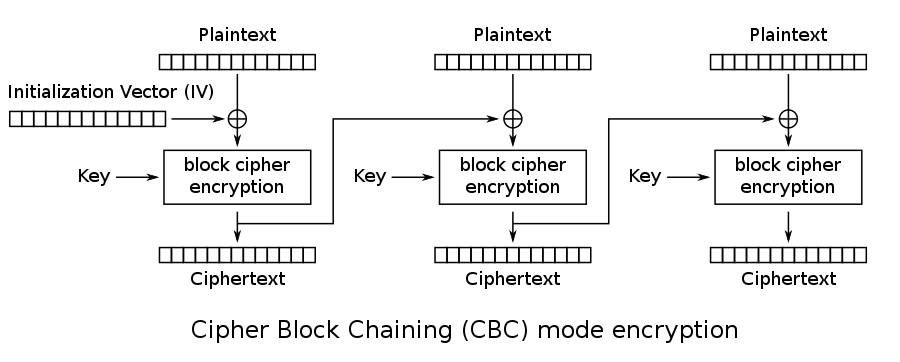
\includegraphics[height=\textheight,width=\textwidth,keepaspectratio]
    {figures/CBC_encryption.png}
    \caption{Cipher Block Chaining (CBC) mode encryption.}\label{fig:cbc_mode}
\end{figure}



\subsection{Using picture {\fontfamily{qcr}\selectfont pic\_original.bmp}}
%
\begin{lstlisting}[language=Bash, caption=Commands generating
    {\fontfamily{qcr}\selectfont pic\_cbc.bmp}, label={lst:pic_cbc}]
$ openssl enc -e -des-cbc -salt -pbkdf2 -kfile password.txt \
    -in pic_original.bmp -out pic_original.bmp.cbc # encrypt the original picture
$ head -c 54 pic_original.bmp > header
$ tail -c +55 pic_original.bmp.cbc > cbc_body
$ cat header cbc_body > pic_cbc.bmp
\end{lstlisting}

\begin{lstlisting}[language=Bash, caption=Commands generating
    {\fontfamily{qcr}\selectfont pic\_ecb.bmp}, label={lst:pic_ecb}]
$ openssl enc -e -des-ecb -salt -pbkdf2 -kfile password.txt \
    -in pic_original.bmp -out pic_original.bmp.ecb # encrypt the original picture
$ head -c 54 pic_original.bmp > header
$ tail -c +55 pic_original.bmp.ecb > ecb_body
$ cat header ecb_body > pic_ecb.bmp
\end{lstlisting}

\begin{figure}
    \centering
    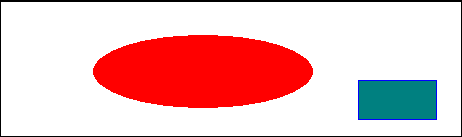
\includegraphics[height=\textheight,width=\textwidth,keepaspectratio]
    {figures/pic_original.png}
    \caption{The original picture.}\label{fig:original_pic}
\end{figure}

\begin{figure}
    \centering
    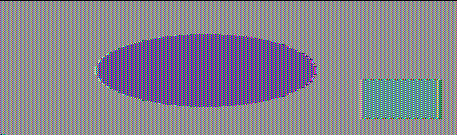
\includegraphics[height=\textheight,width=\textwidth,keepaspectratio]
    {figures/pic_ecb.png}
    \caption{The ECB-mode encrypted picture.}\label{fig:ecb_pic}
\end{figure}

\begin{figure}
    \centering
    
\includegraphics[height=\textheight,width=\textwidth,keepaspectratio]
    {figures/pic_cbc.png}
    \caption{The CBC-mode encrypted picture.}\label{fig:cbc_pic}
\end{figure}

\subsection{Using picture {\fontfamily{qcr}\selectfont snail.bmp}}
%
\begin{lstlisting}[language=Bash, caption=Commands generating
    {\fontfamily{qcr}\selectfont snail\_cbc.bmp}, label={
        lst:snail_cbc
    }]
$ openssl enc -e -des-cbc -salt -pbkdf2 -kfile password.txt \
    -in snail.bmp -out snail.bmp.cbc # encrypt the original picture
$ head -c 54 snail.bmp > snail_header
$ tail -c +55 snail.bmp.cbc > snail_cbc_body
$ cat snail_header snail_cbc_body > snail_cbc.bmp
\end{lstlisting}

\begin{lstlisting}[language=Bash, caption=Commands generating
    {\fontfamily{qcr}\selectfont snail\_ecb.bmp}, label={
        lst:snail_ecb
    }]
$ openssl enc -e -des-ecb -salt -pbkdf2 -kfile password.txt \
    -in snail.bmp -out snail.bmp.ecb # encrypt the original picture
$ head -c 54 snail.bmp > snail_header
$ tail -c +55 snail.bmp.ecb > snail_ecb_body
$ cat snail_header snail_ecb_body > snail_ecb.bmp
\end{lstlisting}

\begin{figure}
    \centering
    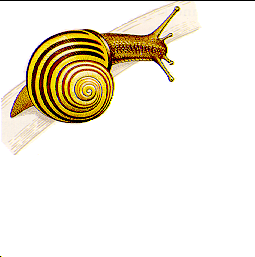
\includegraphics[height=\textheight,width=\textwidth,keepaspectratio]
    {figures/snail.png}
    \caption{The Bitmap picture of a snail.}\label{fig:snail}
\end{figure}

\begin{figure}
    \centering
    
\includegraphics[height=\textheight,width=\textwidth,keepaspectratio]
    {figures/snail_cbc.png}
    \caption{The CBC-mode encrypted picture of a snail.}\label{fig:snail_cbc}
\end{figure}

\begin{figure}
    \centering
    
\includegraphics[height=\textheight,width=\textwidth,keepaspectratio]
    {figures/snail_ecb.png}
    \caption{The ECB-mode encrypted picture of a snail.}\label{fig:snail_ecb}
\end{figure}